%---------------
%╔═╗╔═╗╔╦╗╦ ╦╔═╗
%╚═╗║╣  ║ ║ ║╠═╝
%╚═╝╚═╝ ╩ ╚═╝╩  
%---------------
\documentclass[12pt,oneside,a4paper]{report}

% DOCUMENT SETUP
\usepackage[left=3cm, 
			right=2.5cm, 
			top=2.5cm, 
			bottom=2.5cm, 
			includehead, 
			includefoot]{geometry}

% line spacing
\usepackage{setspace}
\setstretch{1,25} % 15/12 --> 1.25

%de­fines Adobe Times Ro­man as de­fault text font
\usepackage{mathptmx}
\usepackage{times} % needed for acronym package

%PDF linking package
\usepackage[hidelinks]{hyperref}

% Language Setup
\usepackage[ngerman]{babel}
% language specific bibliography style
\usepackage[numbers]{natbib}
\usepackage[fixlanguage]{babelbib}
\selectbiblanguage{german}
% bliographystyle setup
% default style names: apalike alphadin ieeetr IEEEtranSN apalike2 alphadin 
% babel specific: babplain, babplai3, babalpha, babunsrt, bababbrv, bababbr3 unsrt 
\bibliographystyle{unsrturl}

% encoding setup
% T1 font encoding for languages that use a latin alphabet
\usepackage[T1]{fontenc} 

% enhanced input encoding handling - utf8 for äÄüÜöÖß...
\usepackage[utf8]{inputenc}
%\usepackage{ucs}%utf8x suppart

% after babel - set chapter string
\AtBeginDocument{\renewcommand{\chaptername}{}}

% enumeration
\usepackage{enumitem}
% tabular extension tabularx
\usepackage{tabularx}

% math packages
\usepackage{amsmath}
\usepackage{nicefrac}
\usepackage{amsthm}
\usepackage{amsbsy}
\usepackage{amssymb}
\usepackage{amsfonts}
\usepackage{MnSymbol}

% patches for latex
\usepackage{fixltx2e}

%special characters
\usepackage{amssymb}
\usepackage{upgreek,textgreek}

% acronym package
\usepackage[printonlyused, footnote]{acronym}

% breakable text in \seqsplit{}
\usepackage{seqsplit}

% \textmu
\usepackage{textcomp}

% package provides a way to compile sections of a document using the same preamble as the main document
\usepackage{subfiles}

% driver-independent color extension - used by listings,tabularx
\usepackage[usenames,dvipsnames,table,xcdraw]{xcolor}

% -- SYNTAX HIGHLIGHTING --
\usepackage{listings}
%% bash command line Syntax Highlighting
\lstdefinestyle{BASH_CMD}{ 
  columns=fullflexible,            % copy pasteable listings
  language=bash,
  basicstyle=\small\sffamily,
  basicstyle   = \small \ttfamily,
  keywordstyle = [1]\small \ttfamily,
  keywordstyle = [2]\small \ttfamily,
  commentstyle = \small \ttfamily,
  numbers=none,
  captionpos=b, 
  breaklines=true,
  numberstyle=\tiny,
  numbersep=3pt,
  frame=tlrb,
  columns=fullflexible,
  backgroundcolor=\color{white!20},
  linewidth=\linewidth,
  literate=                        % replace in code
     {Ö}{{\"O}}1
     {Ä}{{\"A}}1
     {Ü}{{\"U}}1
     {ß}{{\ss}}2
     {ü}{{\"u}}1
     {ä}{{\"a}}1
     {ö}{{\"o}}1
}
 % adds style BASH_CMD
%% Matlab Syntax Highlighting
\colorlet{keyword}{blue!100!black!80}
\colorlet{STD}{Lavender}
\colorlet{comment}{green!90!black!90}
\definecolor{mygreen}{rgb}{0,0.6,0}
\definecolor{mygray}{rgb}{0.5,0.5,0.5}
\definecolor{mymauve}{rgb}{0.58,0,0.82}


\lstdefinestyle{BASH_SCRIPT}{ 
  language     = bash,
  basicstyle   = \footnotesize \ttfamily,
  keywordstyle = [1]\color{keyword}\bfseries,
  keywordstyle = [2]\color{STD}\bfseries,
  commentstyle = \color{mygreen}\itshape,
  backgroundcolor=\color{white},   % choose the background color; you must add \usepackage{color} 
  columns=fullflexible,            % copy pasteable listings
                                   % or \usepackage{xcolor}
  basicstyle=\footnotesize,        % the size of the fonts that are used for the code
  breakatwhitespace=false,         % sets if automatic breaks should only happen at whitespace
  breaklines=true,                 % sets automatic line breaking
  captionpos=b,                    % sets the caption-position to bottom
  extendedchars=true,              % lets you use non-ASCII characters; for 8-bits encodings only,
                                   % does not work with UTF-8
  frame=single,                    % adds a frame around the code
  keepspaces=true,                 % keeps spaces in text, useful for keeping indentation of code
                                   % (possibly needs columns=flexible)
  numbers=left,                    % where to put the line-numbers; possible values are 
                                   % (none, left, right)
  numbersep=5pt,                   % how far the line-numbers are from the code
  numberstyle=\tiny\color{mygray}, % the style that is used for the line-numbers
  rulecolor=\color{black},         % if not set, the frame-color may be changed on line-breaks
                                   % within not-black text (e.g. comments (green here))
  showspaces=false,                % show spaces everywhere adding particular underscores; it
  	                               % overrides 'showstringspaces'
  showstringspaces=false,          % underline spaces within strings only
  showtabs=false,                  % show tabs within strings adding particular underscores
  stepnumber=1,                    % the step between two line-numbers. If it's 1, each line 
                                   % will be numbered
  stringstyle=\color{mymauve},     % string literal style
  tabsize=2,                       % sets default tabsize to 2 spaces
  title=\lstname,                  % set title name
  literate=                        % replace in code
     {Ö}{{\"O}}1
     {Ä}{{\"A}}1
     {Ü}{{\"U}}1
     {ß}{{\ss}}2
     {ü}{{\"u}}1
     {ä}{{\"a}}1
     {ö}{{\"o}}1
} % adds style BASH_SCRIPT
% Matlab Syntax Highlighting
\colorlet{keyword}{blue!100!black!80}
\colorlet{STD}{red}
\colorlet{comment}{green!90!black!90}
\definecolor{mygreen}{rgb}{0,0.6,0}
\definecolor{mygray}{rgb}{0.5,0.5,0.5}
\definecolor{mymauve}{rgb}{0.58,0,0.82}


\lstdefinestyle{LATEX}{ 
  language     = [LaTeX]{TeX},
  basicstyle   = \footnotesize \ttfamily,
  keywordstyle = [1]\color{keyword}\bfseries,
  keywordstyle = [2]\color{comment}\bfseries,
  commentstyle = \color{mygray}\itshape,
  %backgroundcolor=\color{white},   % choose the background color; you must add \usepackage{color} 
                                   % or \usepackage{xcolor}
  basicstyle=\footnotesize,        		   % the size of the fonts that are used for the code
  breakatwhitespace=false,         % sets if automatic breaks should only happen at whitespace
  columns=fullflexible,            % copy pasteable listings
  breaklines=true,                 % sets automatic line breaking
  captionpos=c,                    % sets the caption-position to bottom
  extendedchars=true,              % lets you use non-ASCII characters; for 8-bits encodings only,
                                   % does not work with UTF-8
  frame=single,                    % adds a frame around the code
  keepspaces=true,                 % keeps spaces in text, useful for keeping indentation of code
                                   % (possibly needs columns=flexible)
  numbers=left,                    % where to put the line-numbers; possible values are 
                                   % (none, left, right)
  numbersep=4pt,                   % how far the line-numbers are from the code
  numberstyle=\tiny\color{mygray}, % the style that is used for the line-numbers
  rulecolor=\color{black},         % if not set, the frame-color may be changed on line-breaks
                                   % within not-black text (e.g. comments (green here))
  showspaces=false,                % show spaces everywhere adding particular underscores; it
  	                               % overrides 'showstringspaces'
  showstringspaces=false,          % underline spaces within strings only
  showtabs=false,                  % show tabs within strings adding particular underscores
  stepnumber=1,                    % the step between two line-numbers. If it's 1, each line 
                                   % will be numbered
  stringstyle=\color{mymauve},     % string literal style
  tabsize=2,                       % sets default tabsize to 2 spaces
  title=\lstname,                  % set title name
  literate=                        % replace in code
     {Ö}{{\"O}}1
     {Ä}{{\"A}}1
     {Ü}{{\"U}}1
     {ß}{{\ss}}2
     {ü}{{\"u}}1
     {ä}{{\"a}}1
     {ö}{{\"o}}1
} % adds style LATEX
%% Matlab Syntax Highlighting
\colorlet{keyword}{blue!100!black!80}
\colorlet{STD}{Lavender}
\colorlet{comment}{green!90!black!90}
\definecolor{mygreen}{rgb}{0,0.6,0}
\definecolor{mygray}{rgb}{0.5,0.5,0.5}
\definecolor{mymauve}{rgb}{0.58,0,0.82}


\lstdefinestyle{MATLAB}{ 
  language     = Matlab,
  basicstyle   = \footnotesize \ttfamily,
  keywordstyle = [1]\color{keyword}\bfseries,
  keywordstyle = [2]\color{STD}\bfseries,
  commentstyle = \color{mygreen}\itshape,
  backgroundcolor=\color{white},   % choose the background color; you must add \usepackage{color} 
                                   % or \usepackage{xcolor}
  basicstyle=\footnotesize,        % the size of the fonts that are used for the code
  breakatwhitespace=false,         % sets if automatic breaks should only happen at whitespace
  columns=fullflexible,            % copy pasteable listings
  breaklines=false,                % sets automatic line breaking
  captionpos=c,                    % sets the caption-position to bottom
  extendedchars=true,              % lets you use non-ASCII characters; for 8-bits encodings only,
                                   % does not work with UTF-8
  frame=single,                    % adds a frame around the code
  keepspaces=true,                 % keeps spaces in text, useful for keeping indentation of code
                                   % (possibly needs columns=flexible)
  numbers=left,                    % where to put the line-numbers; possible values are 
                                   % (none, left, right)
  numbersep=5pt,                   % how far the line-numbers are from the code
  numberstyle=\tiny\color{mygray}, % the style that is used for the line-numbers
  rulecolor=\color{black},         % if not set, the frame-color may be changed on line-breaks
                                   % within not-black text (e.g. comments (green here))
  showspaces=false,                % show spaces everywhere adding particular underscores; it
  	                               % overrides 'showstringspaces'
  showstringspaces=false,          % underline spaces within strings only
  showtabs=false,                  % show tabs within strings adding particular underscores
  stepnumber=1,                    % the step between two line-numbers. If it's 1, each line 
                                   % will be numbered
  stringstyle=\color{mymauve},     % string literal style
  tabsize=2,                       % sets default tabsize to 2 spaces
  title=\lstname,                  % set title name
  literate=                        % replace in code
     {Ö}{{\"O}}1
     {Ä}{{\"A}}1
     {Ü}{{\"U}}1
     {ß}{{\ss}}2
     {ü}{{\"u}}1
     {ä}{{\"a}}1
     {ö}{{\"o}}1
} % adds style MATLAB
% Matlab Syntax Highlighting
\colorlet{keyword}{blue!100!black!80}
\colorlet{STD}{Lavender}
\colorlet{comment}{green!90!black!90}
\definecolor{mygreen}{rgb}{0,0.6,0}
\definecolor{mygray}{rgb}{0.5,0.5,0.5}
\definecolor{mymauve}{rgb}{0.58,0,0.82}


\lstdefinestyle{PYTHON}{ 
  language     = Python,
  basicstyle   = \footnotesize \ttfamily,
  keywordstyle = [1]\color{keyword}\bfseries,
  keywordstyle = [2]\color{STD}\bfseries,
  commentstyle = \color{mygreen}\itshape,
  backgroundcolor=\color{white},   % choose the background color; you must add \usepackage{color} 
                                   % or \usepackage{xcolor}
  basicstyle=\footnotesize,        % the size of the fonts that are used for the code
  columns=fullflexible,            % copy pasteable listings
  breakatwhitespace=false,         % sets if automatic breaks should only happen at whitespace
  breaklines=false,                % sets automatic line breaking
  captionpos=c,                    % sets the caption-position to bottom
  extendedchars=true,              % lets you use non-ASCII characters; for 8-bits encodings only,
                                   % does not work with UTF-8
  frame=single,                    % adds a frame around the code
  keepspaces=true,                 % keeps spaces in text, useful for keeping indentation of code
                                   % (possibly needs columns=flexible)
  numbers=left,                    % where to put the line-numbers; possible values are 
                                   % (none, left, right)
  numbersep=5pt,                   % how far the line-numbers are from the code
  numberstyle=\tiny\color{mygray}, % the style that is used for the line-numbers
  rulecolor=\color{black},         % if not set, the frame-color may be changed on line-breaks
                                   % within not-black text (e.g. comments (green here))
  showspaces=false,                % show spaces everywhere adding particular underscores; it
  	                               % overrides 'showstringspaces'
  showstringspaces=false,          % underline spaces within strings only
  showtabs=false,                  % show tabs within strings adding particular underscores
  stepnumber=1,                    % the step between two line-numbers. If it's 1, each line 
                                   % will be numbered
  stringstyle=\color{mymauve},     % string literal style
  tabsize=2,                       % sets default tabsize to 2 spaces
  title=\lstname,                  % set title name
  literate=                        % replace in code
     {Ö}{{\"O}}1
     {Ä}{{\"A}}1
     {Ü}{{\"U}}1
     {ß}{{\ss}}2
     {ü}{{\"u}}1
     {ä}{{\"a}}1
     {ö}{{\"o}}1
} % adds style PYTHON
%% Matlab Syntax Highlighting
\colorlet{keyword}{blue!100!black!80}
\colorlet{STD}{Lavender}
\colorlet{comment}{green!90!black!90}
\definecolor{mygreen}{rgb}{0,0.6,0}
\definecolor{mygray}{rgb}{0.5,0.5,0.5}
\definecolor{mymauve}{rgb}{0.58,0,0.82}


\lstdefinestyle{CPP}{ 
  language     = C++,
  basicstyle   = \footnotesize \ttfamily,
  keywordstyle = [1]\color{keyword}\bfseries,
  keywordstyle = [2]\color{STD}\bfseries,
  commentstyle = \color{mygreen}\itshape,
  backgroundcolor=\color{white},   % choose the background color; you must add \usepackage{color} 
                                   % or \usepackage{xcolor}
  columns=fullflexible,            % copy pasteable listings
  basicstyle=\footnotesize,        % the size of the fonts that are used for the code
  breakatwhitespace=false,         % sets if automatic breaks should only happen at whitespace
  breaklines=false,                % sets automatic line breaking
  captionpos=c,                    % sets the caption-position to bottom
  extendedchars=true,              % lets you use non-ASCII characters; for 8-bits encodings only,
                                   % does not work with UTF-8
  frame=single,                    % adds a frame around the code
  keepspaces=true,                 % keeps spaces in text, useful for keeping indentation of code
                                   % (possibly needs columns=flexible)
  numbers=left,                    % where to put the line-numbers; possible values are 
                                   % (none, left, right)
  numbersep=5pt,                   % how far the line-numbers are from the code
  numberstyle=\tiny\color{mygray}, % the style that is used for the line-numbers
  rulecolor=\color{black},         % if not set, the frame-color may be changed on line-breaks
                                   % within not-black text (e.g. comments (green here))
  showspaces=false,                % show spaces everywhere adding particular underscores; it
  	                               % overrides 'showstringspaces'
  showstringspaces=false,          % underline spaces within strings only
  showtabs=false,                  % show tabs within strings adding particular underscores
  stepnumber=1,                    % the step between two line-numbers. If it's 1, each line 
                                   % will be numbered
  stringstyle=\color{mymauve},     % string literal style
  tabsize=2,                       % sets default tabsize to 2 spaces
  title=\lstname,                  % set title name
  literate=                        % replace in code
     {Ö}{{\"O}}1
     {Ä}{{\"A}}1
     {Ü}{{\"U}}1
     {ß}{{\ss}}2
     {ü}{{\"u}}1
     {ä}{{\"a}}1
     {ö}{{\"o}}1
} % adds style CPP
%% Matlab Syntax Highlighting
\colorlet{keyword}{blue!100!black!80}
\colorlet{STD}{Lavender}
\colorlet{comment}{green!90!black!90}
\definecolor{mygreen}{rgb}{0,0.6,0}
\definecolor{mygray}{rgb}{0.5,0.5,0.5}
\definecolor{mymauve}{rgb}{0.58,0,0.82}


\lstdefinestyle{C}{ 
  language     = C,
  basicstyle   = \footnotesize \ttfamily,
  keywordstyle = [1]\color{keyword}\bfseries,
  keywordstyle = [2]\color{STD}\bfseries,
  commentstyle = \color{mygreen}\itshape,
  backgroundcolor=\color{white},   % choose the background color; you must add \usepackage{color} 
  columns=fullflexible,            % copy pasteable listings
                                   % or \usepackage{xcolor}
  basicstyle=\footnotesize,        % the size of the fonts that are used for the code
  breakatwhitespace=false,         % sets if automatic breaks should only happen at whitespace
  breaklines=false,                % sets automatic line breaking
  captionpos=c,                    % sets the caption-position to bottom
  extendedchars=true,              % lets you use non-ASCII characters; for 8-bits encodings only,
                                   % does not work with UTF-8
  frame=single,                    % adds a frame around the code
  keepspaces=true,                 % keeps spaces in text, useful for keeping indentation of code
                                   % (possibly needs columns=flexible)
  numbers=left,                    % where to put the line-numbers; possible values are 
                                   % (none, left, right)
  numbersep=5pt,                   % how far the line-numbers are from the code
  numberstyle=\tiny\color{mygray}, % the style that is used for the line-numbers
  rulecolor=\color{black},         % if not set, the frame-color may be changed on line-breaks
                                   % within not-black text (e.g. comments (green here))
  showspaces=false,                % show spaces everywhere adding particular underscores; it
  	                               % overrides 'showstringspaces'
  showstringspaces=false,          % underline spaces within strings only
  showtabs=false,                  % show tabs within strings adding particular underscores
  stepnumber=1,                    % the step between two line-numbers. If it's 1, each line 
                                   % will be numbered
  stringstyle=\color{mymauve},     % string literal style
  tabsize=2,                       % sets default tabsize to 2 spaces
  title=\lstname,                  % set title name
  literate=                        % replace in code
     {Ö}{{\"O}}1
     {Ä}{{\"A}}1
     {Ü}{{\"U}}1
     {ß}{{\ss}}2
     {ü}{{\"u}}1
     {ä}{{\"a}}1
     {ö}{{\"o}}1
} % adds style C
%% JSON Syntax Highlighting
\colorlet{keyword}{blue!100!black!80}
\colorlet{STD}{Lavender}
\colorlet{comment}{green!90!black!90}
\definecolor{mygreen}{rgb}{0,0.6,0}
\definecolor{mygray}{rgb}{0.5,0.5,0.5}
\definecolor{mymauve}{rgb}{0.58,0,0.82}

\newcommand\JSONnumbervaluestyle{\color{blue}}
\newcommand\JSONstringvaluestyle{\color{red}}

\newif\ifcolonfoundonthisline

\makeatletter

\lstdefinelanguage{json}
{
  showstringspaces    = false,
  keywords            = {false,true},
  alsoletter          = 0123456789.,
  morestring          = [s]{"}{"},
  morestring          = [s]{'}{'},
  stringstyle         = \ifcolonfoundonthisline\JSONstringvaluestyle\fi,
  MoreSelectCharTable =%
    \lst@DefSaveDef{`:}\colon@json{\processColon@json},
  basicstyle          = \ttfamily,
  keywordstyle        = \ttfamily\bfseries,
}

% flip the switch if a colon is found in Pmode
\newcommand\processColon@json{
  \colon@json%
  \ifnum\lst@mode=\lst@Pmode%
    \global\colonfoundonthislinetrue%
  \fi
}

\lst@AddToHook{Output}{%
  \ifcolonfoundonthisline%
    \ifnum\lst@mode=\lst@Pmode%
      \def\lst@thestyle{\JSONnumbervaluestyle}%
    \fi
  \fi
  %override by keyword style if a keyword is detected!
  \lsthk@DetectKeywords% 
}

% reset the switch at the end of line
\lst@AddToHook{EOL}%
  {\global\colonfoundonthislinefalse}

\makeatother



\lstdefinestyle{JSON}{ 
  language     = json,
  basicstyle   = \footnotesize \ttfamily,
  keywordstyle = [1]\color{keyword}\bfseries,
  keywordstyle = [2]\color{STD}\bfseries,
  commentstyle = \color{mygreen}\itshape,
  backgroundcolor=\color{white},   % choose the background color; you must add \usepackage{color} 
                                   % or \usepackage{xcolor}
  basicstyle=\footnotesize,        % the size of the fonts that are used for the code
  columns=fullflexible,            % copy pasteable listings
  breakatwhitespace=false,         % sets if automatic breaks should only happen at whitespace
  breaklines=false,                % sets automatic line breaking
  captionpos=c,                    % sets the caption-position to bottom
  extendedchars=true,              % lets you use non-ASCII characters; for 8-bits encodings only,
                                   % does not work with UTF-8
  frame=single,                    % adds a frame around the code
  keepspaces=true,                 % keeps spaces in text, useful for keeping indentation of code
                                   % (possibly needs columns=flexible)
  numbers=left,                    % where to put the line-numbers; possible values are 
                                   % (none, left, right)
  numbersep=5pt,                   % how far the line-numbers are from the code
  numberstyle=\tiny\color{mygray}, % the style that is used for the line-numbers
  rulecolor=\color{black},         % if not set, the frame-color may be changed on line-breaks
                                   % within not-black text (e.g. comments (green here))
  showspaces=false,                % show spaces everywhere adding particular underscores; it
  	                               % overrides 'showstringspaces'
  showstringspaces=false,          % underline spaces within strings only
  showtabs=false,                  % show tabs within strings adding particular underscores
  stepnumber=1,                    % the step between two line-numbers. If it's 1, each line 
                                   % will be numbered
  stringstyle=\color{mymauve},     % string literal style
  tabsize=2,                       % sets default tabsize to 2 spaces
  title=\lstname,                  % set title name
  literate=                        % replace in code
     {Ö}{{\"O}}1
     {Ä}{{\"A}}1
     {Ü}{{\"U}}1
     {ß}{{\ss}}2
     {ü}{{\"u}}1
     {ä}{{\"a}}1
     {ö}{{\"o}}1
} % adds style JSON

% HEADLINE CFG
\usepackage{fancyhdr} % Headers and footers
\usepackage{lastpage}
\usepackage{nopageno}
\setlength{\headheight}{1.5cm}
\pagestyle{fancy} % All pages have headers and footers
\fancyhead{} % Blank out the default header
\fancyfoot{} % Blank out the default footer
\fancyhead[L]{}
\fancyhead[C]{}
\fancyhead[R]{}
\fancyfoot[L]{}
\fancyfoot[C]{\thepage}
\fancyfoot[R]{}
% override plain page style for \part, \chapter or 
% \maketitle, which implicit specifies plain page style
\fancypagestyle{plain} 
{
	\fancyhead[L]{}
	\fancyhead[C]{}
	\fancyhead[R]{}
	\fancyfoot[L]{}
	\fancyfoot[C]{\thepage}
	\fancyfoot[R]{}
}
% set list pagestyle
\fancypagestyle{lists} 
{
	\fancyhead[L]{}
	\fancyhead[C]{}
	\fancyhead[R]{}
	\fancyfoot[L]{}
	\fancyfoot[C]{\thepage}
	\fancyfoot[R]{}
}

\renewcommand{\chaptermark}[1]{\markright{#1}{}}
\renewcommand{\sectionmark}[1]{\markright{#1}{}}
\renewcommand{\headrulewidth}{0pt}
\renewcommand{\footrulewidth}{0pt}

	
\usepackage{verbatim}
\usepackage{graphicx}
\usepackage{epstopdf}

% floating prevention packages
\usepackage{float}    % used with [H] positioning parameter
\usepackage{placeins} % \FloatBarrier 

% tikz packages
\usepackage{tikz}
\usepackage{caption}
\usepackage[list=true,listformat=simple]{subcaption}
\usepackage{standalone}
\usepackage{pgfplots}


% include only specified tex files - uncommend unneeded
\includeonly{preface/cover,
             preface/abstract,
             preface/tableofcontents,
             preface/listoffigures,
             preface/listoftables,
             preface/lstlistoflistings,
             appendix/bibliography}

%-------------------
%╔═╗╔╦╗╦═╗╦╔╗╔╔═╗╔═╗
%╚═╗ ║ ╠╦╝║║║║║ ╦╚═╗
%╚═╝ ╩ ╩╚═╩╝╚╝╚═╝╚═╝
%-------------------
\newcommand{\strLecture}{Signale, Systeme und Sensoren}
\newcommand{\strDate}{\today}
\newcommand{\strAuthorA}{M. Kieser}
\newcommand{\strAuthorB}{J. Altmeyer}
\newcommand{\strAuthorAEmail}{makieser@htwg-konstanz.de}
\newcommand{\strAuthorBEmail}{jualtmey@htwg-konstanz.de}
% Versuchsbeschreibung 
\newcommand{\strTopic}{Aufbau eines einfachen Spracherkenners}
\newcommand{\strAbstract}{ Erstellung eines einfachen Spracherkenners mit dem Prinzip des Prototyp-Klassifikators. Weiterhin wird das Windowing Verfahren behandelt und implementiert. Dieses wird für die Ermittlung der Spektren für den Spracherkenner benötigt.}
% hyperref customization
\hypersetup{
	pdftitle    ={\strTopic}, % title
	pdfsubject	={\strLecture}, % subject of the document
	pdfauthor	={\strAuthorA, \strAuthorB}, % author
	pdfkeywords	={}, % list of keywords
	pdfcreator	={}, % creator of the document
	pdfproducer	={}, % producer of the document
	colorlinks=false, % false: boxed links; true: colored links
	linkcolor=red, % color of internal links (change box color with linkbordercolor)
    citecolor=green, % color of links to bibliography
    filecolor=magenta, % color of file links
    urlcolor=cyan, % color of external links
	%bookmarks=true, % show bookmarks bar?
	unicode=true, % non-Latin characters in Acrobat’s bookmarks
	pdftoolbar=true, % show Acrobat’s toolbar?
	pdfmenubar=true, % show Acrobat’s menu?
    pdffitwindow=false, % window fit to page when opened
	pdfnewwindow=true % links in new PDF window
}

%-----------------------------------------
% ╔╗ ╔═╗╔═╗╦╔╗╔  ╔╦╗╔═╗╔═╗╦ ╦╔╦╗╔═╗╔╗╔╔╦╗ 
% ╠╩╗║╣ ║ ╦║║║║   ║║║ ║║  ║ ║║║║║╣ ║║║ ║  
% ╚═╝╚═╝╚═╝╩╝╚╝  ═╩╝╚═╝╚═╝╚═╝╩ ╩╚═╝╝╚╝ ╩  
%-----------------------------------------

\begin{document}
\pagenumbering{Roman} 

%\setcounter{section}{0}

\begin{titlepage}

\vspace*{-3.5cm}

\begin{flushleft}
\hspace*{-1cm} 
\includegraphics[width=15.7cm]{preface/htwg-logo}
\end{flushleft}

\vspace{1cm}

\begin{center}
	\large{
		\textbf{\strLecture} \\[2cm]
	}
	\Huge{
		\textbf{\strTopic} \\[2cm]
	}
	\Large{
		\textbf{\strAuthorA, \strAuthorB}} \\[3cm]
	\large{
		\textbf{} \\[2.3cm]
	}
	
	\large{
		\textbf{Konstanz, \strDate}
	}
\end{center}

\end{titlepage}
\thispagestyle{empty}




\begin{center}
{\Large \textbf{Zusammenfassung (Abstract)}}
\end{center}

\bigskip

\begin{center}
	\begin{tabular}{p{2.8cm}p{5cm}p{5cm}}
		Thema: & \multicolumn{2}{p{10cm}}{\raggedright\strTopic} \\
		 & & \\
		Autoren: & \strAuthorA & \href{mailto:\strAuthorAEmail}{\strAuthorAEmail} \\
		 & \strAuthorB & \href{mailto:\strAuthorBEmail}{\strAuthorBEmail} \\
		 & & \\
		Betreuer: & Prof. Dr. Matthias O. Franz & \href{mailto:mfranz@htwg-konstanz.de}{mfranz@htwg-konstanz.de} \\
		 &  Jürgen Keppler & \href{mailto:juergen.keppler@htwg-konstanz.de}{juergen.keppler@htwg-konstanz.de} \\
		 &  Martin Miller & \href{mailto:martin.miller@htwg-konstanz.de}{martin.miller@htwg-konstanz.de} \\
	\end{tabular}
\end{center}

\bigskip

\noindent
\strAbstract

\thispagestyle{lists}



\clearpage

%
% TABLE OF CONTENTS
%
\thispagestyle{lists}
%
% TABLE OF CONTENTS
%
\tableofcontents
\thispagestyle{plain}
\newpage

%
% Abbildungsverzeichnis
%
%
% Abbildungsverzeichnis
%
\phantomsection
\addcontentsline{toc}{chapter}{Abbildungsverzeichnis}
\listoffigures
\thispagestyle{lists}
\newpage

%
% Tabellenverzeichnis
%
%
% Tabellenverzeichnis
%
\phantomsection
\addcontentsline{toc}{chapter}{Tabellenverzeichnis}
\listoftables
\thispagestyle{lists}
\newpage

%
% Listingverzeichnis
%
%
% Listingverzeichnis
%
\phantomsection
\renewcommand\lstlistingname{Listing}
\renewcommand\lstlistlistingname{Listingverzeichnis}
\lstlistoflistings
\addcontentsline{toc}{chapter}{Listingverzeichnis}
\thispagestyle{lists}
\newpage


%--------------------------
% ╔═╗╦ ╦╔═╗╔═╗╔╦╗╔═╗╦═╗╔═╗ 
% ║  ╠═╣╠═╣╠═╝ ║ ║╣ ╠╦╝╚═╗ 
% ╚═╝╩ ╩╩ ╩╩   ╩ ╚═╝╩╚═╚═╝ 
%--------------------------

\pagenumbering{arabic} 
\setcounter{page}{1}
%
% CHAPTER Einleitung
%
\chapter{Einleitung}
\label{chap:EINL}
Im nachfolgenden Versuch geht es um die Erstellung eines einfachen Spracherkenners. Dieser wird nach dem Prinzip des Prototyp-Klassifikators umgesetzt. Die zu unterscheidenden Prototypen sind dabei "Hoch", "Tief", "Links", und "Rechts". Der Spracherkenner vergleicht diese im voraus aufgenommenen Prototypen anhand ihres Spektrums mit dem gesprochenen Wort des Benutzers. Bei jedem gesprochenen Wort entscheidet der Spracherkenner wie stark das Wort mit einem der Prototypen korreliert.
Der Spracherkenner wählt den Prototypen, wo es zu der größten Übereinstimmung kommt. \\
Für den Vergleich der Spektren benötigt man die Windowing Methode, welche in Kapitel \ref{chap:VERSUCH_1} vorbereitend behandelt wird.
Der eigentliche Spracherkenner wird in Kapitel \ref{chap:VERSUCH_2} erstellt.



%
% CHAPTER Versuch 1
%
\chapter{Versuch 1- Fourieranalyse lang andauernder Signale}
\label{chap:VERSUCH_1}

Lang andauernde Signale sind für die Fourieranalyse sehr rechenintensiv. Deshalb bedient man sich der Methode des Windowing, welches nach Franz2015 \cite{Franz2015i} das Signal in oft überlappende Fenster zerlegt. Diese Zerlegung ermöglicht eine lokale Fourieranalyse eines Fensters. Diese Analyse ist wesentlich schneller durchgeführt, da man nur einen Teil des Signals betrachtet.
In dem nachfolgenden Versuch wird die Windowing Methode implementiert und anschließend auf ihre Korrektheit anhand eines Beispiel Signals geprüft.

\section{Fragestellung, Aufbau, Messprinzip, Messmittel}
\label{chap:VERSUCH_1_FRAGESTELLUNG}
\textbf{Fragestellung:} Ist das Amplitudenspektrum eines Audiosignals durch die Windowing Methode richtig dargestellt.\\
\textbf{Aufbau:} Der Antwort auf diese Frage wird sich in 5 Schritten genähert:

a) automatisierte Aufnahme eines Audiosignals und dessen Speicherung

b) Aufbereitung des Audiosignals durch Triggerung und Zeitangleichung

c) Erstellung des Amplitudenspektrums des Audiosignals

d) Anwendung des Windowing-Verfahrens  auf das Audiosignal

e) Vergleich der Beiden Amplitudenspektren in Kapitel \ref{chap:VERSUCH_1_INTERPRETATION} \\\\
\textbf{Messprinzip und Messmittel:} Es wird ein Mikrofon als Messmittel eingesetzt. Das Mikrofon erzeugt je nach empfangenen Ton einen entsprechenden Spannungswert. Mithilfe dieses Messprinzips lassen sich die Informationen weiterverarbeiten. 

\section{Messwerte}
\label{chap:VERSUCH_1_MESSWERTE}
Nachfolgend die Messwerte zu den Schritten a) und b):

\begin{figure}[H]
\centering\small
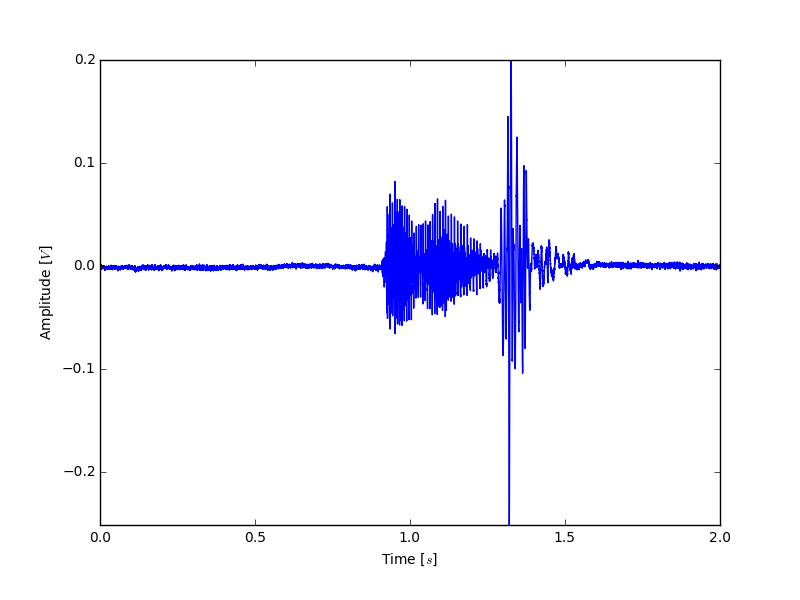
\includegraphics [scale=0.8]{src/v1.png}
\caption{ \textbf{a)} unbearbeitetes Audiosignal des Wortes <<Aua>>}
\label{fig:AUA_unbearbeitet}
\end{figure}

\begin{figure}[H]
\centering\small
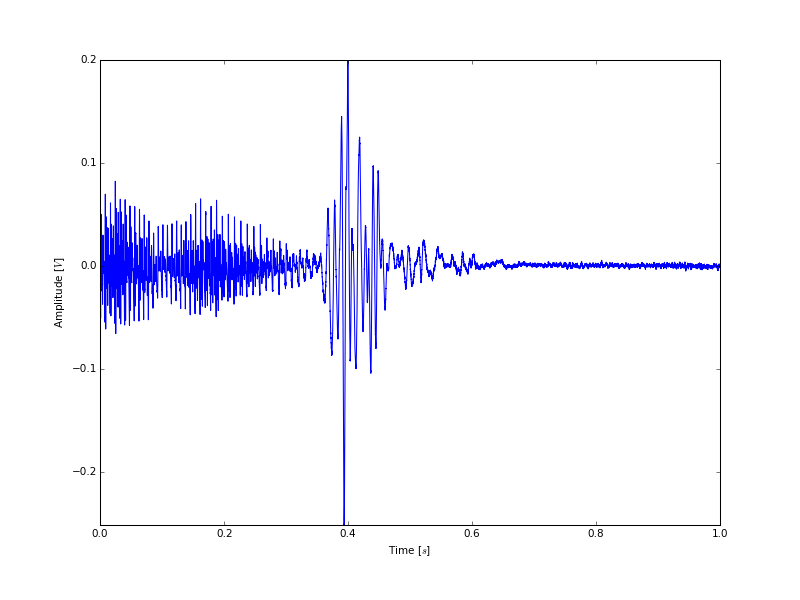
\includegraphics [scale=0.45]{src/Aufnahme1TriggerCut.png}
\caption{ \textbf{b)} aufbereitetes Audiosignal aus a), getriggert und eine Sekunde lang}
\label{fig:AUA_TriggerCut}
\end{figure}


\section{Auswertung}
\label{chap:VERSUCH_1_AUSWERTUNG}
\textbf{Schritt c)}\\
Aus dem aufbereiteten Audiosignal aus Abbildung \ref{fig:AUA_TriggerCut} wird mittels der Fouriertransformation das Amplitudenspektrum in Abbildung \ref{fig:AUA_TriggerCutFFT} erzeugt. Dabei wird das ganze Signal komplett betrachtet. Die Berechnung der Ergebnisse sind dem Pythoncode in Listing \ref{lst:Code} zu entnehmen.\\
\textbf{Schritt d)}\\
Verglichen zu dem in Schritt c) berechneten Amplitudenspektrum, wird nun das Amplitudenspektrum aus mehreren Teilbereichen mittels der Windowing Methode zusammengestellt. Die Zusammenführung des Signals entsteht durch Mittlung der einzelnen Teilbereiche. Das Ergebnis ist in Abbildung \ref{fig:AUA_TriggerCutWindow} dargestellt.
Die Berechnung des Windowing sind speziell der Methode <<windowing(rec)>> aus Listing \ref{lst:Code} zu entnehmen.

\begin{figure}[H]
\centering\small
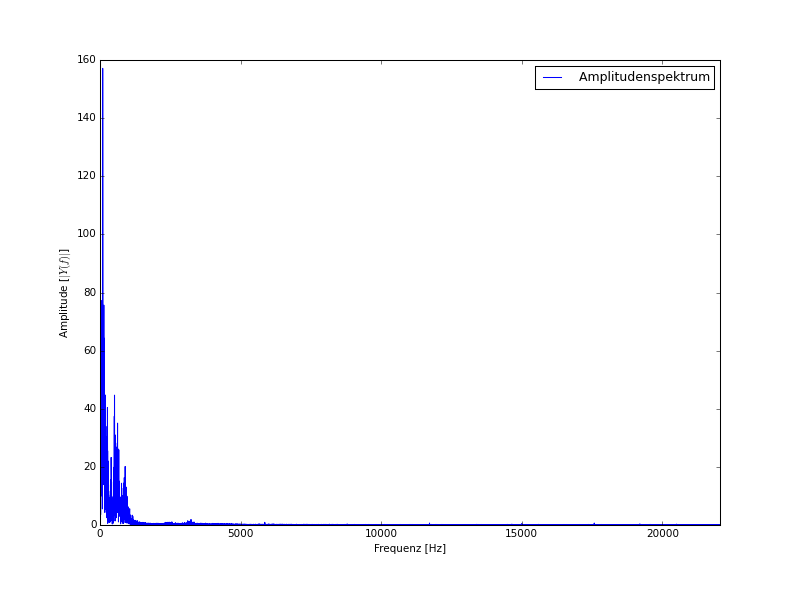
\includegraphics [scale=0.45]{src/Aufnahme1TriggerCutFFT.png}
\caption{ \textbf{c)} Amplitudenspektrum des aufbereiteten Audiosignals}
\label{fig:AUA_TriggerCutFFT}
\end{figure}

\begin{figure}[H]
\centering\small
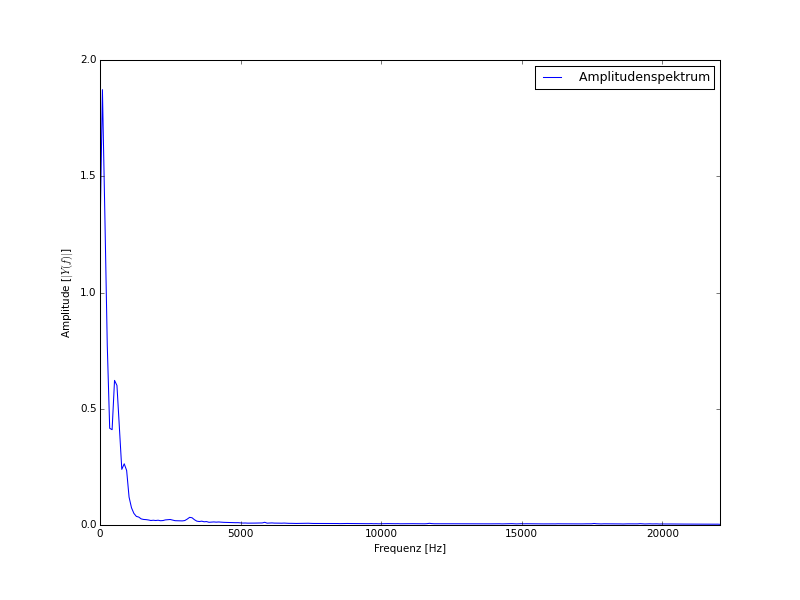
\includegraphics [scale=0.45]{src/Aufnahme1TriggerCutWindow.png}
\caption{ \textbf{d)} Amplitudenspektrum nach Windowing des aufbereiteten Audiosignals}
\label{fig:AUA_TriggerCutWindow}
\end{figure}



\section{Interpretation}
\label{chap:VERSUCH_1_INTERPRETATION}
In Abbildung \ref{fig:AUA_TriggerCutWindow} sieht man einen geglätteten Verlauf des in Abbildung \ref{fig:AUA_TriggerCutFFT} gezeigten Amplitudenspektrums.
Vergleicht man nun Abbildung \ref{fig:AUA_TriggerCutFFT} und Abbildung \ref{fig:AUA_TriggerCutWindow} so erkennt man, dass die Amplitudenspektren vom  Profil einander entsprechen. Dies zeigt die korrekte Berechnung der Windowing Methode. 

%
% CHAPTER Versuch 2
%
\chapter{Versuch 2 - Spracherkennung}
\label{chap:VERSUCH_2}

Dieser Versuch zeigt die Funktionsweise eines einfachen Spracherkenners.
Dazu wird ein Spracherkenner so aufgebaut, dass er die Worte ''Hoch'', ''Tief'', ''Links'' und ''Rechts'' erkennt. Mit diesen Befehlen könnte beispielsweise ein Gabelstapler in einem Hochregallager sprachgesteuert werden. Der Spracherkenner basiert auf dem Prinzip des Prototyp-Klassifikators, wie es in der Vorlesung 10 von Herrn Franz \cite{Franz2015i} beschrieben ist.

\section{Fragestellung, Messprinzip, Aufbau, Messmittel}
\label{chap:VERSUCH_2_FRAGESTELLUNG}

Wie ist ein Spracherkenner aufgebaut und wie funktioniert er?
Antworten darauf liefern die folgenden Kapitel, insbesondere Kapitel \ref{chap:VERSUCH_2_AUSWERTUNG}.

\paragraph{}

Für den Spracherkenner wird ein Referenzspektrum bzw. einen Prototyp für jedes Wort, welches er später erkennen soll, benötigt. Zudem ist es sinnvoll einen Testdatensatz aufzunehmen.
Dazu wird der selbe Versuchsaufbau wie in Versuch 1 verwendet.
Mit dem Mikrofon wird diesmal ein Referenzdatensatz und ein Testdatensatz von zwei Sprechern A und B aufgenommen.
Der Referenzdatensatz besteht aus den Worten ''Hoch'', ''Tief'', ''Links'' und ''Rechts'', jeweils fünf mal, von Sprecher A gesprochen. Dieser dient dem Spracherkenner später als Vergleichswert. Der Testdatensatz besteht ebenfalls aus den oben genannten Worten, jeweils fünf mal, einmal von Sprecher A und einmal von Sprecher B gesprochen.

\section{Messwerte}
\label{chap:VERSUCH_2_MESSWERTE}

Alle in Kapitel \ref{chap:VERSUCH_2_FRAGESTELLUNG} gemachten Aufnahmen (Referenzsignale und Testsignale) sind getriggert und auf die Länge von einer Sekunde zu geschnitten.
Für die Testsignale ist an dieser Stelle keine weitere Bearbeitung notwendig.
Das Referenzspektrum für später soll jedoch schon hier berechnet werden.
Dazu wird auf jedes Referenzsignal die Windowing-Methode aus Versuch 1 angewandt.
Das Referenzspektrum für jedes Wort erhalten wir durch zusätzliche Mittelung der jeweils fünf Spektren.
In den Abbildungen \ref{fig:REF_HOCH}, \ref{fig:REF_TIEF}, \ref{fig:REF_LINKS} und  \ref{fig:REF_RECHTS} ist jeweils das Referenzspektrum der Worte ''Hoch'', ''Tief'', ''Links'' und ''Rechts'' abgebildet.

\begin{figure}[H]
\centering\small
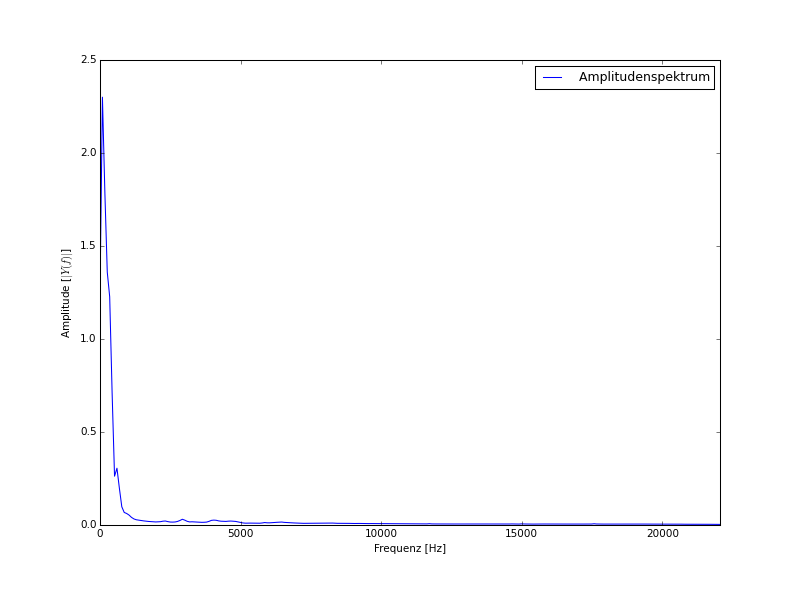
\includegraphics[scale=0.5]{src/ReferenzspektrumHoch.png}
\caption{Referenzspektrum des Wortes "Hoch"}
\label{fig:REF_HOCH}
\end{figure}

\begin{figure}[H]
\centering\small
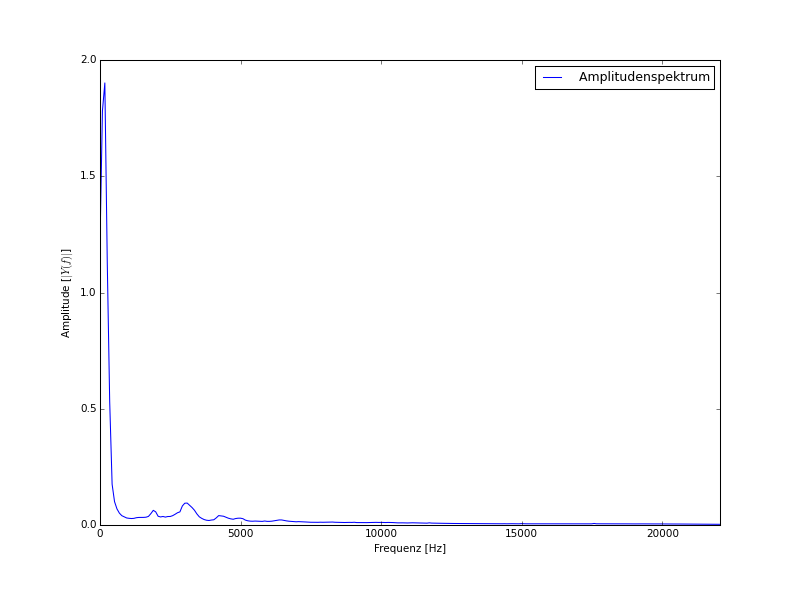
\includegraphics[scale=0.5]{src/ReferenzspektrumTief.png}
\caption{Referenzspektrum des Wortes "Tief"}
\label{fig:REF_TIEF}

\centering\small
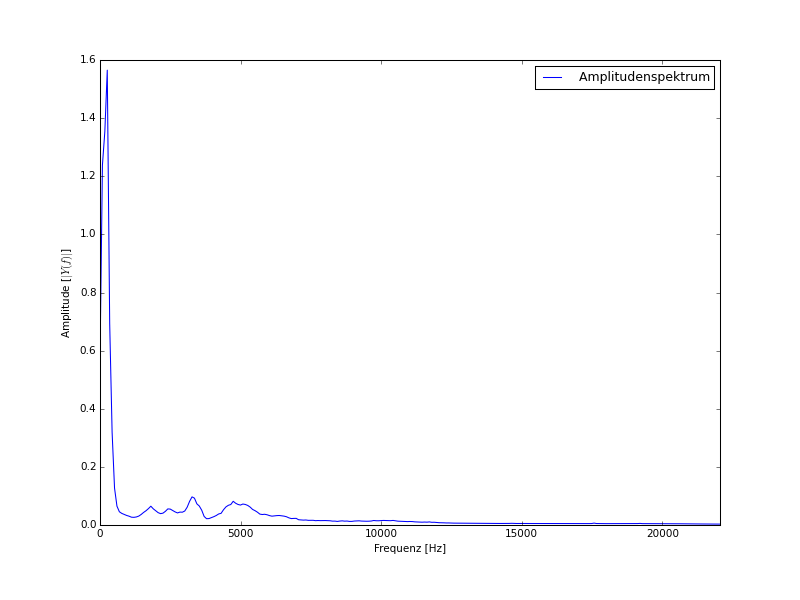
\includegraphics[scale=0.5]{src/ReferenzspektrumLinks.png}
\caption{Referenzspektrum des Wortes "Links"}
\label{fig:REF_LINKS}
\end{figure}

\begin{figure}[H]
\centering\small
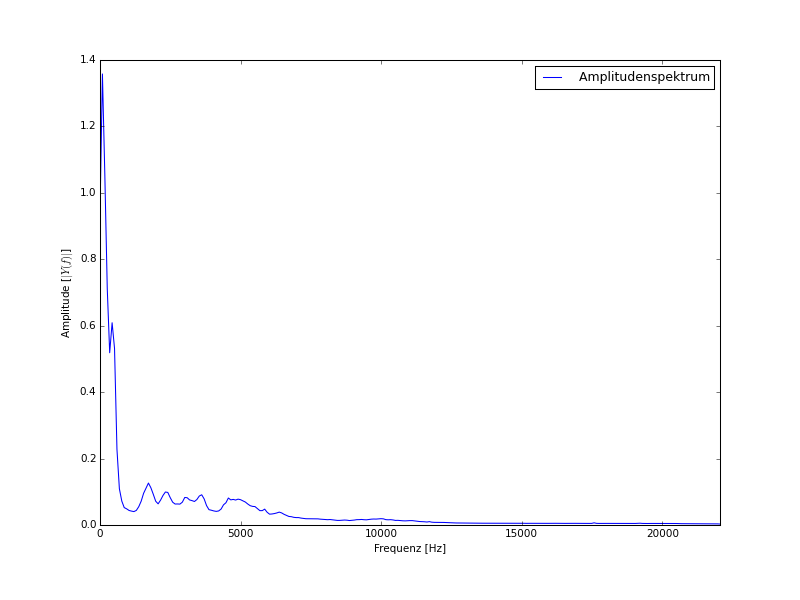
\includegraphics[scale=0.5]{src/ReferenzspektrumRechts.png}
\caption{Referenzspektrum des Wortes "Rechts"}
\label{fig:REF_RECHTS}
\end{figure}

\section{Auswertung}
\label{chap:VERSUCH_2_AUSWERTUNG}

Mit den Messwerten aus Kapitel \ref{chap:VERSUCH_2_MESSWERTE} kann nun ein Spracherkenner aufgebaut und getestet werden.
Unser Spracherkenner funktioniert folgendermaßen:

\paragraph{}

Ein beliebiges Signal (also ein Wort) aus dem Testdatensatz wird dem Spracherkenner übergeben. Dieser berechnet zunächst das Spektrum des Signals mit der Windowing-Methode.
Danach vergleicht bzw. korreliert er jedes Referenzspektrum mit dem Eingabespektrum. Dazu wird jeweils der Korrelationskoeffizient nach Bravais-Pearson berechnet. Ein Koeffizient nahe an 1 bedeutet eine hohe Ähnlichkeit der Signale, nahe an 0 das Gegenteil. Der Spracherkenner entscheidet sich nun für das Wort, welches die höchste Übereinstimmung mit einem der Referenzspektren hat, d.h. das Wort bei dem der Korrelationskoeffizient insgesamt betrachtet am größten ist.
In Python wurde dafür eine Methode speechRecognition() erstellt, siehe Listing \ref{chap:APPENDIX_SOURCECODE}.

\paragraph{}

Um den oben gezeigten Spracherkenner zu testen, werden ihm alle Testspektren übergeben. Das bedeutet jeweils fünf mal die Worte ''Hoch'', ''Tief'', ''Links'' und ''Rechts'' einmal von Sprecher A und einmal von Sprecher B gesprochen.
Die Tabelle \ref{tab:DETEKTIONSRATE} zeigt nun die Detektionsrate unseres Spracherkenners für das jeweilige Wort pro Sprecher. Insgesamt ergibt sich eine Detektionsrate von 1.0 für Sprecher A und 0.5 für Sprecher B.

\begin{table}[H]
\centering 
\begin{tabular}{ccc}
\hline
\textbf{Wort} &\textbf{Sprecher A} & \textbf{Sprecher B} \\
\hline
Hoch & 1.0 & 0.6 \\
\hline
Tief & 1.0 & 0.4 \\
\hline
Links & 1.0 & 0.0 \\
\hline
Rechts & 1.0 & 1.0 \\
\hline
\end{tabular} 
\caption{Detektionsraten des Spracherkenners für das jeweilige Wort}
\label{tab:DETEKTIONSRATE}
\end{table}

\section{Interpretation}
\label{chap:VERSUCH_2_INTERPRETATION}

Wie die Tabelle \ref{tab:DETEKTIONSRATE} zeigt, funktioniert der Spracherkenner hervorragend für Sprecher A. Alle Wörter wurden richtig erkannt. Von Sprecher A stammen jedoch auch die Referenzspektren, wodurch dieses Ergebnis nicht besonders überrascht.
Bei Sprecher B schneidet der Spracherkenner eher schlecht ab. Lediglich das Wort ''Rechts'' wurde immer korrekt erfasst, das Wort ''Links'' wurde sogar nie erkannt.
Der Spracherkenner arbeitet nur für Sprecher A zuverlässig.

%
% CHAPTER Anhang
%
\renewcommand\thesection{A.\arabic{section}}
\renewcommand\thesubsection{\thesection.\arabic{subsection}}

\chapter*{Anhang}
\label{chap:APPENDIX}
\addcontentsline{toc}{chapter}{Anhang}
%\setcounter{chapter}{0}
\addtocounter{chapter}{1}
\setcounter{section}{0}

\section{Quellcode für Versuche 1 - 2}
\label{chap:APPENDIX_SOURCECODE}
\begin{lstlisting}[style=PYTHON, frame=single, caption=QuellCodeV1 bis V2, captionpos=b, label=lst:Code]

#-*-coding:utf-8-*-
"""
CreatedonMonDec714:09:282015

@author:edc10
"""

#import pyaudio
import numpy as np
import scipy.signal as win
import scipy.stats as stats
import matplotlib.pyplot as plt

#FORMAT = pyaudio.paInt16
SAMPLEFREQ = 44100
SEC=2
READBYTES = int(44100*SEC)
TRIGGER = 800
WINDOWSIZE = 512
WINDOWTIME = WINDOWSIZE / SAMPLEFREQ


def plotRecord(rec, filename=''):
    myDpi = 75
    fig, ax = plt.subplots(figsize=(800/myDpi, 600/myDpi), dpi=myDpi)
    ax.autoscale(enable=True, axis='x', tight=True)
    time = np.linspace(0, len(rec)/SAMPLEFREQ, len(rec))
    amp = rec/((2**15)-1)
    ax.plot(time, amp)
    ax.set_xlabel('Time [$s$]')
    ax.set_ylabel('Amplitude [$V$]')
    if filename is not '':
        fig.savefig(filename, transparent=True, dpi=myDpi)
    return
    
    
def trigger(rec):
    for i in range(len(rec)):
        if rec[i] > TRIGGER:
            return rec[i:]
    return []


def cut(rec):
    if len(rec) < SAMPLEFREQ:
        size = SAMPLEFREQ - len(rec)
        rec = np.append(rec, np.zeros(size))

    return rec[:SAMPLEFREQ]


def getInputDataPyAudio():
    p = pyaudio.PyAudio()
    print('running')
    
    stream = p.open(format=FORMAT, channels=1, rate=SAMPLEFREQ,
                    input=True, frames_per_buffer=READBYTES)
    data = stream.read(READBYTES)
    decoded = np.fromstring(data, 'Int16')

    stream.stop_stream()
    stream.close()
    p.terminate()
    print('done')
    return decoded


def plotFFT(rec, filename=''):
    
    #fft
    # n = Anzahl der Schwingungen innerhalb der gesamten Signaldauer
    amp = rec/((2**15)-1)
    c = np.fft.fft(amp)
    n = np.abs(c)
    
    # spiegelung eleminieren
    half = len(n)/2+1
    #print(half)
    count = np.arange(0, int(half))
    #print(count)
    
    # Anzahl der Schwingungen innerhalb der gesamten Signaldauer dargestellt
    dpi=75
    fig, axN = plt.subplots(figsize=(800/dpi,600/dpi), dpi=dpi)
    axN.plot(count[:],n[:half], color = "blue", label=" Amplitudenspektrum ")
    # lässt X-Achse bei 0 beginnen
    axN.autoscale(enable=True, axis='x', tight=True)
    axN.legend(loc='upper right');
    axN.set_xlabel("Frequenz [Hz]")
    axN.set_ylabel("Amplitude [$|Y(f)|$]")
    
    # als png abspeichern    
    if filename is not '':
        fig.savefig(filename, transparent=True, dpi=dpi)
    return


def plotFFT2(rec, filename=''):  
    # spiegelung eleminieren
    half = len(rec)/2+1
    count = np.arange(0, int(half)) / WINDOWTIME
    
    # Anzahl der Schwingungen innerhalb der gesamten Signaldauer dargestellt
    dpi=75
    fig, axN = plt.subplots(figsize=(800/dpi,600/dpi), dpi=dpi)
    axN.plot(count[:],rec[:half], color = "blue", label=" Amplitudenspektrum ")
    # lässt X-Achse bei 0 beginnen
    axN.autoscale(enable=True, axis='x', tight=True)
    axN.legend(loc='upper right');
    axN.set_xlabel("Frequenz [Hz]")
    axN.set_ylabel("Amplitude [$|Y(f)|$]")
    
    # als png abspeichern    
    if filename is not '':
        fig.savefig(filename, transparent=True, dpi=dpi)
    return


def record5():
    for i in range(5):
        data = getInputDataPyAudio()
        triggered = trigger(data)
        cutted = cut(triggered)
        plotRecord(cutted)
        np.savetxt("TestMarcelRechts" + str(i) + ".csv", cutted, delimiter=",")
        print("fertig")
        input()
    return


def getInputData(filename):
    return np.genfromtxt(filename, delimiter=',')


def windowing(rec):
    # Inrervalle für die Windows berechnen
    steps = []
    for i in range(0, len(rec), int(WINDOWSIZE / 2)):
        steps.append(i)
    steps.append(len(rec))

    # Windows erstellen
    windows = []
    for i in range(len(steps) - 3):
        windows.append(rec[steps[i]:steps[i + 2]])

    #----------------------------------------------------

    # Gaus anwenden
    for i in range(len(windows)):
        windows[i] = windows[i] * win.gaussian(WINDOWSIZE, std=WINDOWSIZE/4)
    
    # lokale Fouriertransformation
    result = np.zeros(WINDOWSIZE)
    for i in range(len(windows)):
        windows[i] = np.fft.fft(windows[i]/((2**15)-1))
        windows[i] = np.abs(windows[i])
        result = result + windows[i]
    
    result = result / len(windows)
    return result


def getMeans(pathname):
    files = ['Hoch', 'Tief', 'Links', 'Rechts']
    dic = {}
    for name in files:
        result = []
        for i in range(5):
            data = getInputData(pathname + name + str(i) + ".csv")
            result.append(windowing(data))
    
        summ = np.zeros(WINDOWSIZE)
        for res in result:
            summ = summ + res
        
        mean = summ / len(result)
        dic[name] = mean
    return dic


def speechRecognition(referenceDict, data):
    data = windowing(data)
    maximum = 0
    for key in referenceDict:
        coefficient = stats.pearsonr(referenceDict[key], data)[0]
        if coefficient > maximum:
            maximum = coefficient
            bestKey = key
    return bestKey


def versuch1a():
    decoded = getInputDataPyAudio()
    #np.savetxt("Aufnahme1.csv", decoded, delimiter=",")
    plotRecord(decoded)
    #plotRecord(decoded, 'v1.png')


def versuch1b():
    decoded = getInputDataPyAudio()
    triggered = trigger(decoded)
    cutted = cut(triggered)
    plotRecord(cutted)


def versuch1bc():
    data = np.genfromtxt('Aufnahme1.csv', delimiter=',')
    triggered = trigger(data)
    cutted = cut(triggered)
    plotRecord(cutted, 'Aufnahme1TriggerCut.png')
    np.savetxt("Aufnahme1TriggerCut.csv", cutted, delimiter=",")
    plotFFT(cutted, 'Aufnahme1TriggerCutFFT.png')


def versuch1d():
    data = getInputData('Aufnahme1TriggerCut.csv')
    data = windowing(data)
    plotFFT2(data, "Aufnahme1TriggerCutWindow")


def versuch2():
    # Referenzspektrum einlesen (Prototypen)
    reference = getMeans("Referenz/Referenz")

    # Testdaten in Dictionaries abspeichern
    testJulian = {}
    testMarcel = {}
    for name in ['Hoch', 'Tief', 'Links', 'Rechts']:
        testJulian[name] = []
        testMarcel[name] = []
        for i in range(5):
            dataJulian = getInputData("TestJulian/TestJulian" + name + str(i) + ".csv")
            dataMarcel = getInputData("TestMarcel/TestMarcel" + name + str(i) + ".csv")
            testJulian[name].append(dataJulian)
            testMarcel[name].append(dataMarcel)
    
    #Referenzspektren plotten
    for key in reference:
        plotFFT2(reference[key], 'Referenzspektrum' + key + ".png")
    
    # Spracherkennung
    print("---Julian---")
    for key in testJulian:
        detections = 0
        for i in range(5):
            word = speechRecognition(reference, testJulian[key][i])
            print("Wort:" + key)
            print("Erkannt: " + word)
            if word == key:
                detections += 1
        detectionRate = detections / 5
        print("Detektionsrate " + key + ": " + str(detectionRate))

    print()

    print("---Marcel---")
    for key in testMarcel:
        detections = 0
        for i in range(5):
            word = speechRecognition(reference, testMarcel[key][i])
            print("Wort:" + key)
            print("Erkannt: " + word)
            if word == key:
                detections += 1
        detectionRate = detections / 5
        print("Detektionsrate " + key + ": " + str(detectionRate))


def main():
    #versuch1a()
    #versuch1bc()
    #record5()
    #versuch1d()
    versuch2()


if __name__ == "__main__":
    main()

\end{lstlisting}

%
% Literaturverzeichnis
%
%
% Literaturverzeichnis
%
\phantomsection
\addcontentsline{toc}{chapter}{Literaturverzeichnis}
\bibliography{../references}
\newpage

\end{document}
%------------------------------------
% ╔═╗╔╗╔╔╦╗  ╔╦╗╔═╗╔═╗╦ ╦╔╦╗╔═╗╔╗╔╔╦╗
% ║╣ ║║║ ║║   ║║║ ║║  ║ ║║║║║╣ ║║║ ║ 
% ╚═╝╝╚╝═╩╝  ═╩╝╚═╝╚═╝╚═╝╩ ╩╚═╝╝╚╝ ╩ 
%------------------------------------